\documentclass{article}

\usepackage{graphicx}
\usepackage{tikz}
\usepackage{tikzsymbols}
\usetikzlibrary{calc,patterns,shapes.geometric}
\pagestyle{empty}
\usepackage[margin=0pt]{geometry}
\geometry{papersize={14in,12in}}

\def\centerarc[#1](#2)(#3:#4:#5){\draw[#1] ($(#2)+({#5*cos(#3)},{#5*sin(#3)})$) arc (#3:#4:#5);}

\begin{document}
	\begin{figure}
		\centering
		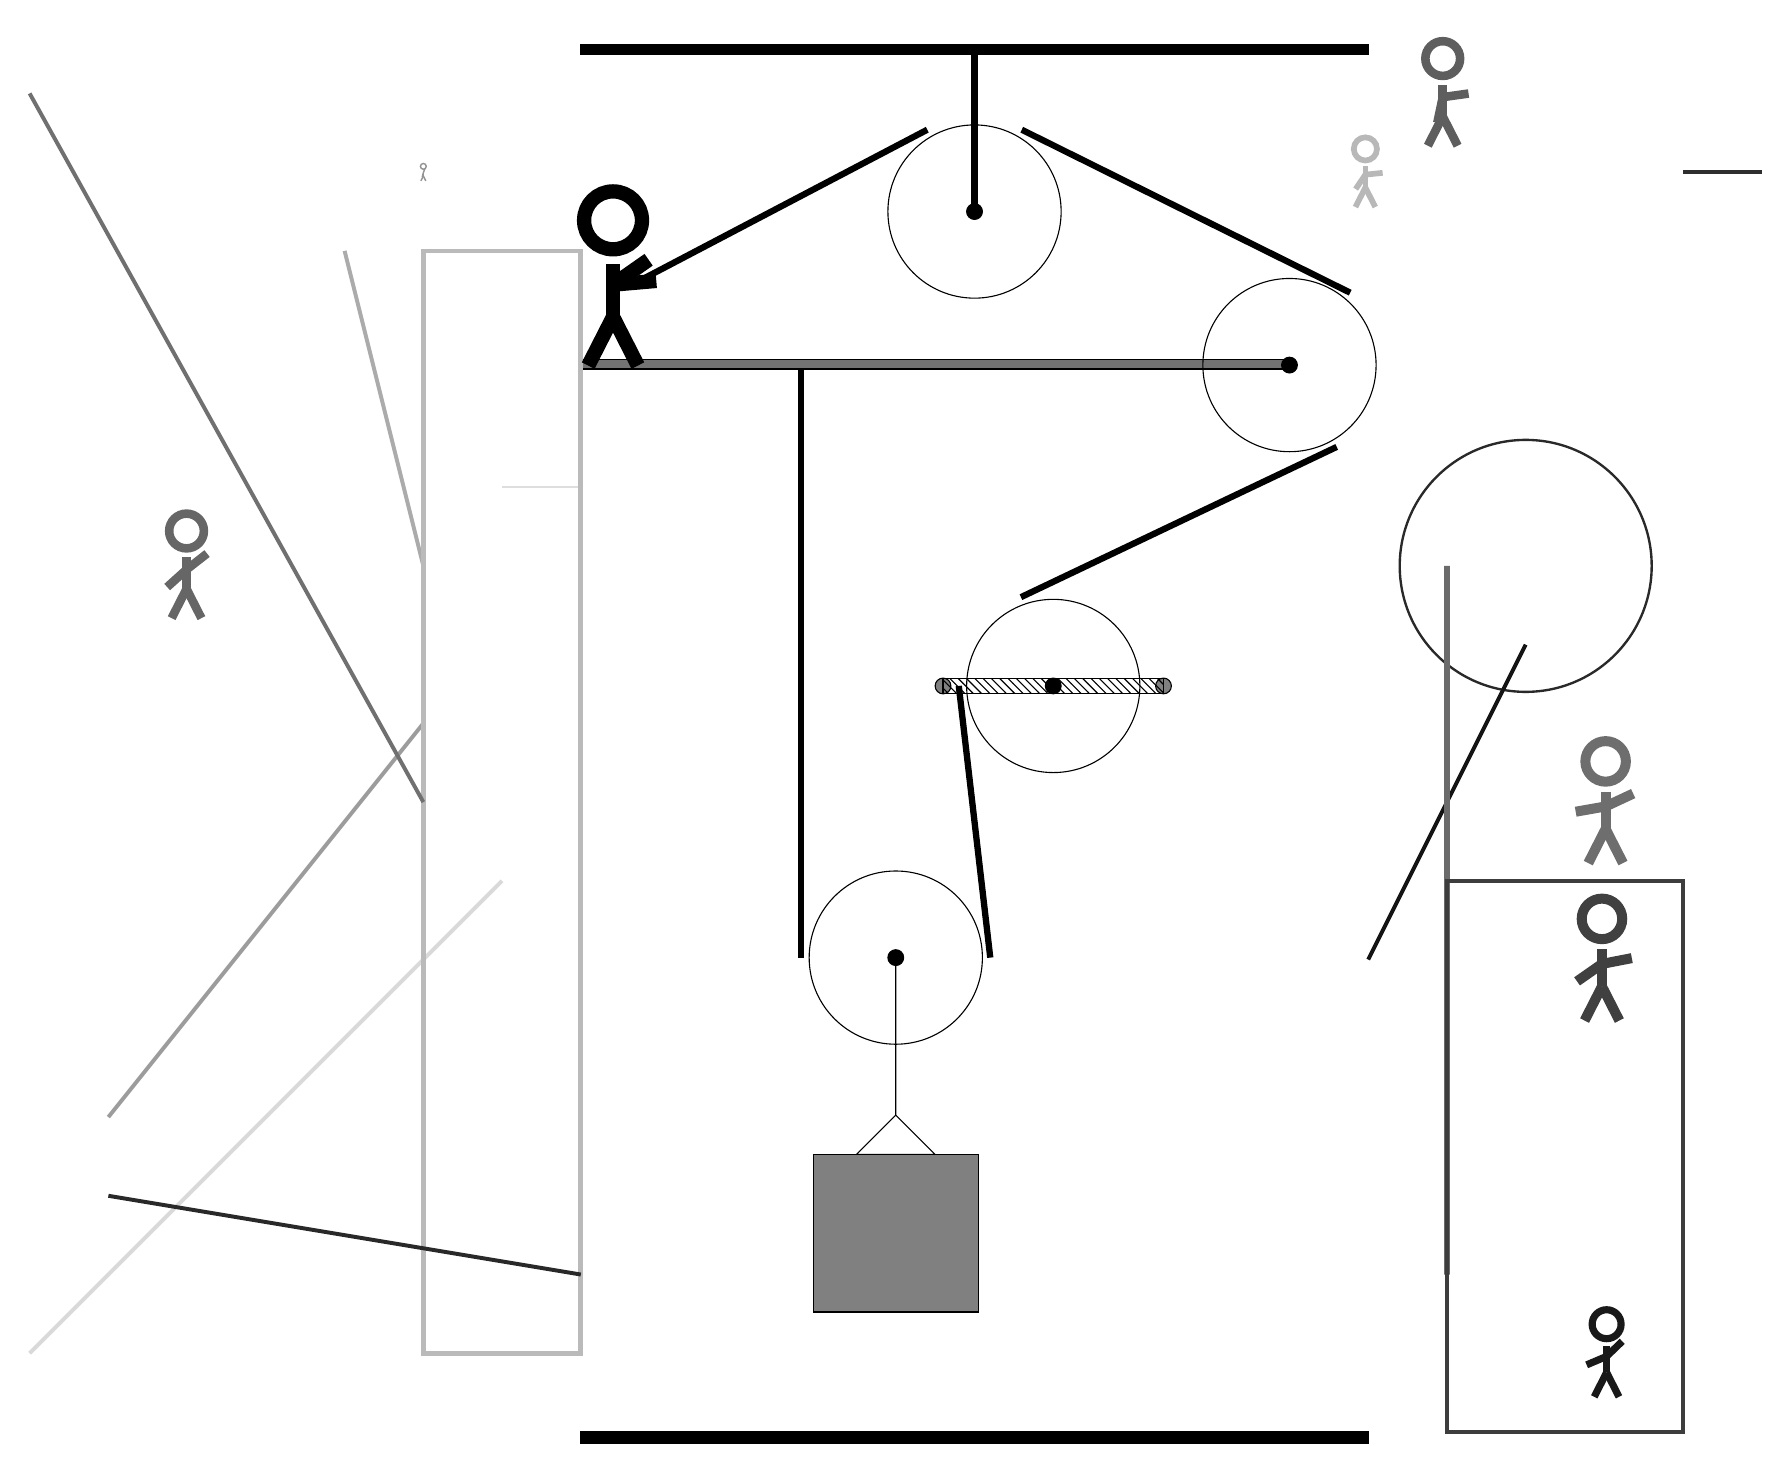
\begin{tikzpicture}
			%%%%% START %%%%%
			
			\draw[fill=black] (-2, 15.5) rectangle (8, 15.625);
			
			\draw[fill=black!55] (-2, 11.5) rectangle (7, 11.625);
			
			\draw (2, 4.025) circle (1.1);
			\draw[fill=black] (2, 4.025) circle (0.1);
			
			\draw (7, 11.55) circle (1.1);
			\draw[fill=black] (7, 11.55) circle (0.1);
			
			\draw[fill=white](4, 7.475) circle (1.1);
			\draw[fill=black] (4, 7.475) circle (0.1);
			\draw[fill=black!50] (2.6, 7.475) circle (0.1);
			\draw[fill=black!50] (5.4, 7.475) circle (0.1);
			\draw[pattern=north west lines, pattern color=black] (2.6, 7.575) rectangle (5.4, 7.375);
			
			\draw (3, 13.5) circle (1.1);
			\draw[fill=black] (3, 13.5) circle (0.1);
			\draw[line width=0.8mm] (3, 13.5) -- (3, 15.5);
			
			\draw (2, 4.025) -- (2, 2.025) -- (1.5, 1.525) -- (2.5, 1.525) -- (2, 2.025);
			\draw[fill=black!50] (0.95, 1.525) rectangle (3.05, -0.475);
			
			\draw[line width=0.8mm] (0.8, 11.5) -- (0.8, 4.025);
			\centerarc[line width=0.8mm](2, 4.025)(180:360:1.2000000000000002);
			\draw[line width=0.8mm](3.2, 4.025) -- (2.8, 7.475);
			\centerarc[line width=0.8mm](4, 7.475)(110:180:1.2000000000000002);
			\draw[line width=0.8mm](3.5896, 8.6026) -- (7.6, 10.5108);
			\centerarc[line width=0.8mm](7, 11.55)(-60:50:1.2000000000000002);
			\draw[line width=0.8mm](7.7714, 12.4692) -- (3.6, 14.5392);
			\centerarc[line width=0.8mm](3, 13.5)(60:120:1.2000000000000002);
			\draw[line width=0.8mm](2.4, 14.5392) -- (-1.2, 12.65);
			
			\draw [line width=0.5mm, color=black!94](10, 11) circle (0.0);
			
			\node[line width=0.3mm, color=black!63] at (9, 15) {\Strichmaxerl[6][78][8]};
			\draw[line width=0.5mm, color=black!82](13, 14) -- (12, 14);
			\node[line width=0.4mm, color=black!60] at (-7, 9) {\Strichmaxerl[6][42][38]};
			\draw [line width=0.3mm, color=black!84](10, 9) circle (1.6);
			
			\node[line width=0.4mm, color=black!57] at (11, 6) {\Strichmaxerl[7][10][25]};
			\draw[line width=0.5mm, color=black!39](-4, 7) -- (-8, 2);
			\node[line width=0.6mm, color=black!75] at (11, 4) {\Strichmaxerl[7][35][11]};
			\draw[line width=0.5mm, color=black!92](8, 4) -- (10, 8);
			\node[line width=0.2mm, color=black!90] at (11, -1) {\Strichmaxerl[5][23][44]};
			\draw[line width=0.7mm, color=black!58] (9, 0) rectangle (9, 9);
			\node[line width=0.6mm, color=black!28] at (8, 14) {\Strichmaxerl[4][56][6]};
			\draw[line width=0.3mm, color=black!13] (-3, 10) rectangle (-2, 10);
			
			\node[line width=0.7mm, color=black!42] at (-4, 14) {\Strichmaxerl[1][76][70]};
			\draw[line width=0.5mm, color=black!15](-3, 5) -- (-9, -1);
			\draw[line width=0.5mm, color=black!33](-5, 13) -- (-4, 9);
			
			\draw[line width=0.6mm, color=black!27] (-2, 13) rectangle (-4, -1);
			\draw[line width=0.5mm, color=black!84](-2, 0) -- (-8, 1);
			\draw[line width=0.5mm, color=black!76] (9, 5) rectangle (12, -2);
			\draw[line width=0.5mm, color=black!56](-4, 6) -- (-9, 15);
			
			\node at (-1.5, 12.65) {\Strichmaxerl[10][-175][35]};
			
			\draw[fill=black] (-2, -2) rectangle (8, -2.15);
			
			%%%%% END %%%%%
		\end{tikzpicture}
	\end{figure}	
\end{document}